\section{Nonconvex functions}

\begin{marginfigure}
    \centering
    \incfig{local-minimum}
    \caption{Gradient descent may get stuck in a local minimum $\vec{y}^\star \neq \vec{x}^\star$, in nonconvex functions.}
    \label{fig:local-minimum}
\end{marginfigure}

\begin{marginfigure}
    \centering
    \incfig{saddle-point}
    \caption{Gradient may get stuck in a flat region (saddle point) in nonconvex functions.}
    \label{fig:saddle-point}
\end{marginfigure}

\begin{marginfigure}
    \centering
    \incfig{no-critical-point}
    \caption{Gradient descent may never even reach a critical point in nonconvex functions.}
    \label{fig:no-critical-point}
\end{marginfigure}

So far, all convergence results that we have proved have been for variants of gradient descent on
convex functions. The reason for this is that, in general, we cannot expect gradient descent to
come close to the global minimum $\vec{x}^\star$ of nonconvex functions.
\Cref{fig:local-minimum,fig:saddle-point,fig:no-critical-point} show what can go wrong in nonconvex
functions, under the assumption that we have set the $\gamma$ such that we do not overshoot. These
figures show points that gradient descent cannot escape; local minima and saddle points.
Furthermore, it might even be that gradient descent never converges to a critical point; see
\Cref{fig:no-critical-point}.

In practice, gradient descent works well on the nonconvex functions that we care about. But,
theoretical explanations for this are mostly missing. Despite this, we will show that under
favorable conditions, we can still say something useful about the behavior of gradient descent on
nonconvex functions.

We can easily make an analysis of gradient descent on smooth functions. A useful property that we
will use is that functions with bounded Hessians are smooth, as shown in the following lemma.

\begin{lemma}
    Let $f: \dom{f} \to \R$ be twice differentiable with $\mathcal{X} \in \dom{f}$ a convex set and
    $\| \hess{f(\vec{x})}{} \| \leq L$ for all $\vec{x} \in \mathcal{X}$. Then $f$ is smooth with
    parameter $L$ over $\mathcal{X}$.
\end{lemma}

\begin{proof}
    Bounded Hessians imply Lipschitz continuity of the gradient, \[
        \| \grad{f(\vec{x})}{} - \grad{f(\vec{y})}{} \| \leq L \| \vec{x} - \vec{y} \|, \quad \forall \vec{x},\vec{y}\in\mathcal{X}.
    \]
    We will use the fundamental theorem of calculus with \[
        h(t) \doteq f(\vec{x} + t(\vec{y} - \vec{x})), \quad t \in [0,1].
    \]
    The derivative can be calculated by chain rule, \[
        h'(t) = \transpose{\grad{f(\vec{x} + t(\vec{y} - \vec{x}))}{}} (\vec{y} - \vec{x}).
    \]
    Now, we can show smoothness,
    \begin{align*}
         & f(\vec{y}) - f(\vec{x}) - \transpose{\grad{f(\vec{x})}{}}(\vec{y}-\vec{x})                                                                                                                    \\ & = h(1) - h(0) - \transpose{\grad{f(\vec{x})}{}} (\vec{y} - \vec{x}) \margintag{Definition of $h$.}                                                                                            \\
         & = \int_0^1 h'(t) \mathrm{d}t - \transpose{\grad{f(\vec{x})}{}} (\vec{y} - \vec{x}) \margintag{Fundamental theorem of calculus.}                                                               \\
         & = \int_0^1 \transpose{\grad{f(\vec{x} + t(\vec{y} - \vec{x}))}{}} (\vec{y} - \vec{x}) \mathrm{d}t - \transpose{\grad{f(\vec{x})}{}} (\vec{y} - \vec{x}) \margintag{Fill in $h'(t)$.}          \\
         & = \int_0^1 \transpose{\grad{f(\vec{x} + t(\vec{y} - \vec{x}))}{}} (\vec{y} - \vec{x}) - \transpose{\grad{f(\vec{x})}{}} (\vec{y} - \vec{x}) \mathrm{d}t \margintag{Integral from $0$ to $1$.} \\
         & = \int_0^1 \transpose{(\grad{f(\vec{x} + t(\vec{y} - \vec{x}))}{} - \grad{f(\vec{x})}{})} (\vec{y} - \vec{x}) \mathrm{d}t                                                                     \\
         & \leq \int_0^1 \lft| \transpose{(\grad{f(\vec{x} + t(\vec{y} - \vec{x}))}{} - \grad{f(\vec{x})}{})} (\vec{y} - \vec{x}) \rgt| \mathrm{d}t                                                      \\
         & \leq \int_0^1 \| \grad{f(\vec{x} + t(\vec{y} - \vec{x}))}{} - \grad{f(\vec{x})}{} \| \| \vec{y} - \vec{x} \| \mathrm{d}t \margintag{Cauchy-Schwarz inequality.}                               \\
         & \leq \int_0^1 L \| t(\vec{y} - \vec{x}) \| \| \vec{y} - \vec{x} \| \mathrm{d}t \margintag{Lipschitz continuous gradient.}                                                                     \\
         & = \int_0^1 Lt \| \vec{x} - \vec{y} \|^2 \mathrm{d}t                                                                                                                                           \\
         & = \frac{L}{2} \| \vec{x} - \vec{y} \|^2.
    \end{align*}
    Thus, we have smoothness, \[
        f(\vec{y}) \leq f(\vec{x}) + \transpose{\grad{f(\vec{x})}{}} (\vec{y} - \vec{x}) + \frac{L}{2} \| \vec{x} - \vec{y} \|^2.
    \]
\end{proof}

Now, we can use this fact and sufficient decrease\sidenote{Recall that sufficient decrease did not
    require convexity.} to prove that the gradients of smooth functions are bounded and approach 0, as
we increase the number of iterations.

\begin{theorem}
    Let $f: \R^d \to \R$ be differentiable with a global minimum $\vec{x}^\star$. Furthermore, suppose that $f$ is smooth with parameter $L$. Choosing stepsize \[
        \gamma \doteq \frac{1}{L},
    \]
    gradient descent yields \[
        \frac{1}{T} \sum_{t=0}^{T-1} \| \grad{f(\vec{x}_t)}{} \|^2 \leq \frac{2L}{T} (f(\vec{x}_0) - f(\vec{x}^\star)).
    \]
\end{theorem}

\begin{remark}
    Note that concave functions are not a counter example to this theorem, despite their gradients
    growing, because they have no global minimum $\vec{x}^\star$.
\end{remark}

\begin{proof}
    Recall that sufficient decrease does not require convexity, \[
        f(\vec{x}_{t+1}) \leq f(\vec{x}_t) - \frac{1}{2L} \| \grad{f(\vec{x}_t)}{} \|^2.
    \]
    Rewriting this, we get \[
        \| \grad{f(\vec{x}_t)}{} \|^2 \leq 2L (f(\vec{x}_t) - f(\vec{x}_{t+1})).
    \]
    Then, by telescoping sum, we get \[
        \sum_{t=0}^{T-1} \| \grad{f(\vec{x}_t)}{} \|^2 \leq 2L (f(\vec{x}_0) - f(\vec{x}_T)) \leq 2L (f(\vec{x}_0) - f(\vec{x}^\star)).
    \]
    The statement follows by dividing both sides by $T$.
\end{proof}

This has the result that \[
    \lim_{t \to \infty} \| \grad{f(\vec{x}_t)}{} \|^2 = 0.
\]
It might seem that convergence of the gradients to 0 is the same as convergence to a critical
point. But, this interpretation does not hold in general; see \Cref{fig:no-critical-point}. In this
case, the gradient converges to 0, but the iterates only move further away from the critical point.
So, this is not a very strong result.

\subsection{Trajectory analysis}

Despite the fact that a nonconvex function may contain local minima, saddle points, and flat parts,
gradient descent may avoid them and still converge to a global minimum. For this, you need a good
starting point and do a trajectory analysis. As an example, we will do a trajectory analysis for a
simplified deep linear neural network. It turns out that this function is smooth along the
trajectories that we analysis, and this is the most important ingredient of the analysis.

\marginnote{Note that stacking linear layers has no benefit, since any stacking of linear layers can
    be represented by a single linear layer. However, the reason for doing this is that it gives us a
    simple playground in which we can try to understanding why training deep neural networks with
    gradient descent works, despite the fact that the objective function is nonconvex.}

Let \[
    \vec{\theta} = \{ \mat{W}_1, \ldots, \mat{W}_{\ell} \}
\]
be the weights of the deep linear network. And, in general, we want to approximate a matrix
$\mat{Y}$, given input matrix $\mat{X}$. Thus, we want to minimize \[
    \| \mat{W}_\ell \mat{W}_{\ell-1} \cdots \mat{W}_{1} \mat{X} - \mat{Y} \|_F^2.
\]

\cite{arora2018convergence} consider this general framework, but we will only consider the case where
all matrices are $1\times 1$, \ie, scalars. Assume we have training input $x = 1$ and output $y = 1$, then we have the following function to optimize, \[
    f(\vec{x}) \doteq \frac{1}{2} \lft( \prod_{k=1}^d x_k - 1 \rgt)^2. \margintag{We rewrite $\vec{w}$ as $\vec{x}$ and $\ell$ as $d$ to be more in line with the notation used here.}
\]
We can immediately see that setting $x_k=1$ for all $k$ minimizes the function at 0. However, we
want to know whether gradient descent will also be able to find this set of weights.

The gradient of this function is computed by \[
    \grad{f(\vec{x})}{i} = \lft( \prod_{k=1}^d x_k - 1 \rgt) \prod_{k\neq i}^{d} x_k
\]
Whenever at least two dimensions are zero, the gradient vanishes. Thus, any $\vec{x}$ with two zero
entries are critical points, despite not being global minima, since then the product of all entries
must be 1, which is not possible if at least two are zero.\sidenote{This shows that $f$ is
    nonconvex, since local minima are global minima in convex functions.} We know that the value of all
such saddle points is $\nicefrac{1}{2}$.

\begin{marginfigure}
    \centering
    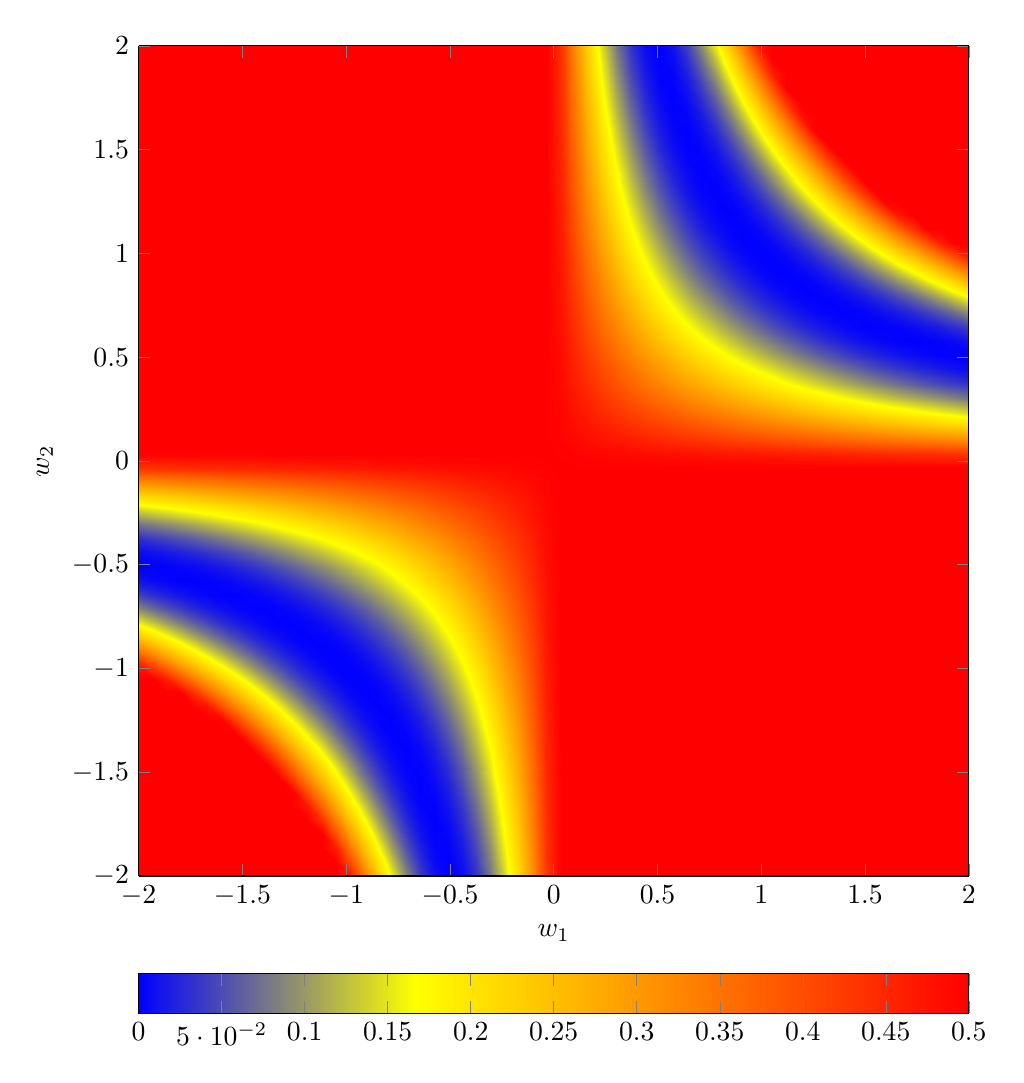
\begin{tikzpicture}
        \begin{axis}[
                width=\textwidth,
                height=\textwidth,
                domain=-2:2,
                y domain=-2:2,
                zmin=0,
                zmax=0.5,
                xlabel=$w_1$,
                ylabel=$w_2$,
                view={0}{90},
                samples=60,
                colorbar,
                colorbar horizontal,
            ]
            \addplot3[
                surf,
                shader=interp,
                point meta=z,
                point meta max=0.5,
                point meta min=0,
            ]{((x * y - 1)^2) / 2};
        \end{axis}
    \end{tikzpicture}
    \caption{$f(\vec{x}) = \frac{1}{2} \lft( \prod_k x_k - 1 \rgt)^2$ for $d=2$, where the loss is clipped to be at most $\nicefrac{1}{2}$.}
    \label{fig:deep-linear-loss-landscape}
\end{marginfigure}

We now want to show that for any number of layers (\ie dimensionality of $\vec{x}$), anywhere in
$\mathcal{X} = \lft\{ \vec{x} \;\middle|\; \vec{x} > \vec{0}, \prod_{k=1}^{d} x_k \leq 1 \rgt\}$,
despite that $f$ is not smooth over $\mathcal{X}$. However, we only need to show that $f$ is smooth
along the trajectory of gradient descent for suitable $L$, so that we get sufficient decrease. We
will now show this by showing that the Hessians over the trajectory are bounded. The Hessian is
given by \[
    \hess{f(\vec{x})}{ij} = \begin{cases}
        \lft( \prod_{k\neq i}^d x_k \rgt)^2,                                         & j = i     \\
        2 \prod_{k\neq i}^{d} x_k \prod_{k\neq j}^d x_k - \prod_{k\neq i,j}^{d} x_k, & j \neq i.
    \end{cases}
\]

\begin{definition}[$c$-balanced.]
    Let $\vec{x} > \vec{0}$ and $c \geq 1$. $\vec{x}$ is called $c$-balanced if $x_i \leq cx_j$ for
    all $1 \leq i,j \leq d$.
\end{definition}

\begin{lemma}
    Let $\vec{x} > \vec{0}$ be $c$-balanced with $\prod_k x_k \leq 1$, then for any stepsize
    $\gamma > 0$, $\vec{x}' \doteq \vec{x} - \gamma \grad{f(\vec{x})}{}$ satisfies $\vec{x}' \geq
        \vec{x}$ componentwise, and is also $c$-balanced.
\end{lemma}

\begin{proof}
    Let \[
        \Delta \doteq -\gamma \lft( \prod_{k=1}^d x_k - 1 \rgt) \lft( \prod_{k=1}^d x_k \rgt) \geq 0.
    \]
    Then, \[
        -\gamma \grad{f(\vec{x})}{k} = \frac{\Delta}{x_k}.
    \]
    Thus, the gradient descent update has the following form, \[
        x'_k = x_k + \frac{\Delta}{x_k} \geq x_k, \quad k \in [d].
    \]
    For all $i,j$, we thus get \[
        x_i' = x_i + \frac{\Delta}{x_i} \leq c x_j + \frac{c \Delta}{x_j} = cx'_j. \margintag{$x_j \leq cx_i \iff \frac{1}{x_i} \leq \frac{c}{x_j}$.}
    \]
\end{proof}

So, we know now that all iterates are $c$-balanced if $\vec{x}_0$ is balanced with $c$. We can use
this to compute a bound on the Hessian by bounding the products.

\begin{lemma}
    Suppose $\vec{x} > \vec{0}$ is $c$-balanced. Then, for any $I \subseteq [d]$, we have \[
        \prod_{k \not\in I} x_k \leq c^{|I|} \lft( \prod_{k=1}^d x_k \rgt)^{1- \nicefrac{|I|}{d}} \leq c^{|I|}.
    \]
\end{lemma}

\begin{proof}
    For any $i\in [d]$, we have $c^d \cdot x_i^d \geq \prod_k x_k$ by
    $c$-balancedness, hence $x_i \geq \frac{1}{c} \lft( \prod_k x_k \rgt)^{\nicefrac{1}{d}}$. Thus, \[
        \prod_{k \not\in I} x_k = \frac{\prod_{k} x_k}{\prod_{i \in I} x_i} \leq \frac{\prod_{k} x_k}{(\nicefrac{1}{c})^{|I|} \lft( \prod_{k} x_k \rgt)^{\nicefrac{|I|}{d}}} = c^{|I|} \lft( \prod_{k=1}^{d} x_k \rgt)^{1-\nicefrac{|I|}{d}}.
    \]
    Since $\prod_k x_k \leq 1$, we can bound the above by $c^{|I|}$.
\end{proof}

\begin{lemma}
    Let $\vec{x} > \vec{0}$ be $c$-balanced with $\prod_k x_k \leq 1$, then \[
        \lft\| \hess{f(\vec{x})}{} \rgt\| \leq \lft\| \hess{f(\vec{x})}{} \rgt\|_F \leq 3 d c^2.
    \]
\end{lemma}

\begin{proof}
    The fact that $\| \mat{A} \| \leq \| \mat{A} \|_F$ is well known. To bound the Frobenius norm, we
    use the previous lemma to compute \[
        \lft|\hess{f(\vec{x})}{ii}\rgt| = \lft| \lft( \prod_{k \neq i} x_i \rgt)^2 \rgt| \leq c^2,
    \]
    and for $i \neq j$, we get \[
        \lft| \hess{f(\vec{x})}{ij} \rgt| \leq \lft| 2 \prod_{k \neq i} x_k \prod_{k \neq j} x_k \rgt| + \lft| \prod_{k\neq i,j} x_k \rgt| \leq 3c^2.
    \]
    Thus, \[
        \| \hess{f(\vec{x})}{} \|_F^2 \leq 9d^2 c^4.
    \]
    Taking the square root, the statement follows.
\end{proof}

This lemma implies smoothness of $f$ with parameter $L=3dc^2$ along the whole trajectory of
gradient descent, under the ``smooth stepsize'' $\gamma \doteq \nicefrac{1}{L} =
    \nicefrac{1}{3dc^2}$. Now, we can use this to prove convergence.

\begin{theorem}
    Let $c \geq 1$ and $\delta < 0$ such that $\vec{x}_0 > \vec{0}$ is $c$-balanced with
    $\delta \leq \prod_k (\vec{x}_0)_k < 1$. Choosing stepsize \[
        \gamma \doteq \frac{1}{3dc^2},
    \]
    gradient descent satisfies \[
        f(\vec{x}_T) \leq \lft( 1- \frac{\delta^2}{3c^4} \rgt)^T f(\vec{x}_0).
    \]
\end{theorem}

\begin{proof}
    For each $t \geq 0$, $f$ is smooth over $\mathrm{conv}(\{ \vec{x}_t, \vec{x}_{t+1} \})$ with
    parameter $L = 3dc^2$, hence we have sufficient decrease, \[
        f(\vec{x}_{t+1}) \leq f(\vec{x}_t) - \frac{1}{6dc^2} \| \grad{f(\vec{x}_t)}{} \|^2.
    \]
    For every $c$-balanced $\vec{x}$ with $\delta \leq \prod_k x_k \leq 1$, we have
    \begin{align*}
        \| \grad{f(\vec{x}_t)}{} \|^2 & = 2f(\vec{x}) \sum_{i=1}^{d} \lft( \prod_{k \neq i} x_k \rgt)^2                      \\
                                      & \geq 2 f(\vec{x}) \frac{d}{c^2} \lft( \prod_{k=1}^{d} x_k \rgt)^{2- \nicefrac{2}{d}} \\
                                      & \geq 2 f(\vec{x}) \frac{d}{c^2} \lft( \prod_{k=1}^{d} x_k \rgt)^2                    \\
                                      & \geq 2 f(\vec{x}) \frac{d}{c^2} \delta^2.
    \end{align*}
    Hence, \[
        f(\vec{x}_{t+1}) \leq f(\vec{x}_t) - \frac{1}{6dc^2} 2 f(\vec{x}_t) \frac{d}{c^2}\delta^2 = f(\vec{x}_t) \lft( 1 - \frac{\delta^2}{3c^4} \rgt).
    \]
\end{proof}

Thus, we seem to have fast convergence, since the function value goes down by a constant factor in
each step. However, there is a catch. Consider the $\vec{x}_0 = [\nicefrac{1}{2}, \ldots,
    \nicefrac{1}{2}]$, which is $c$-balanced with $c=1$, and $\delta = \nicefrac{1}{2^d}$. Hence, the
constant factor is \[
    1 - \frac{1}{3\cdot 4^d}.
\]
This means that we would need $T \approx 4^d$ iterations to reduce the initial error by a constant
factor not depending on $d$. Hence, for this starting value, the gradient is exponentially small.
In order to get polynomial convergence, we need to start with a $\delta$ that decays at most
polynomially with $d$. For large $d$, this has the consequence that we must start very close to
optimality. In particular, we need to start at a distance $\bigo{\nicefrac{1}{\sqrt{d}}}$ from the
optimal solution $[1, \ldots, 1]$.
